\label{sec:results}
% Consequences and implications for the public policy from different expected results.
\subsection{Results for wholesale}
\label{subsec:r_wholesale}
For wholesale consumers the baseline specification \eqref{eq:baseline} is first estimated separately for each hour of the business day to identify peak, off-peak, and the shoulder hours as seen in figure \ref{fig:ws_elasticity_hour}. Based on these estimates the peak-period is defined as the five consecutive hours 11-15 (between the red lines) for all of which the estimated elasticity $\widehat{\varepsilon}$ is below $-.045$, while the off-peak period is defined as the five consecutive hours 00-04 (between the green lines) where $\widehat{\varepsilon}$ is greater than $-.030$. The hours on each side of these intervals are classified as shoulder periods. For non-business days none of these classifications are used because the estimated elasticities do not vary much, they are all of small magnitude ($\widehat{\varepsilon}\geq-.03$)  and even insignificant for several hours of the day.
\begin{figure}[H]
  \centering
  \caption{log wholesale electricity consumption by hour, business days (REIV)}
    \label{fig:ws_elasticity_hour}
  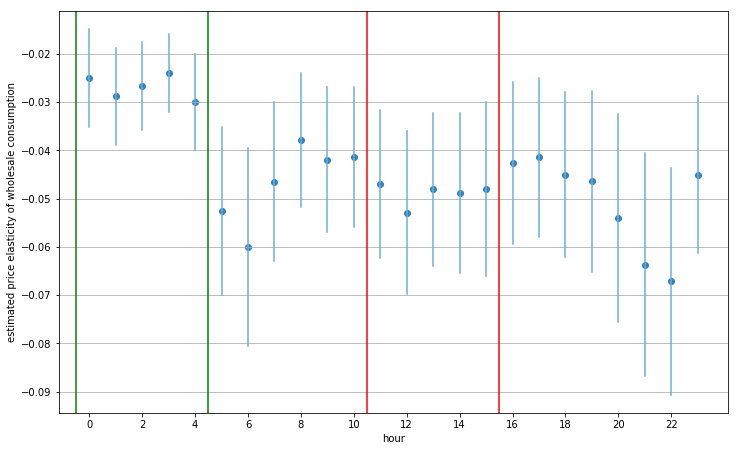
\includegraphics[width=1 \textwidth]{03_figures/ws_elasticity_hour}
\end{figure}
As we find there is almost no difference between the FE and RE estimates (appendix \ref{app:hausman}) the Hausman statistic \eqref{eq:hausman} is low enough that we clearly reject exogeneity of unobserved effects and use REIV for consistent and efficient estimation of the quasi-time-demeaned system of our model \eqref{eq:baseline} and the reduced form \eqref{eq:reduced}.
\bigskip\par
For each of the above mentioned classifications table \ref{tab:ws_preferred} show the REIV estimates of wholesale electricity consumption which is instrumented for by wind power prognosis for the same region. As can be noted from column 1 for the peak-hours 11-15 on business days, wholesale of electricity is estimated to decrease with almost 5 percent when the spot price doubles all other things equal. As seen in table \ref{tab:descriptive} the overall standard deviation of 108 DKK is a deviation by 43 percent of mean price, thus an increase in the price by a full standard deviation would decrease electricity demand by 2 percent.
\par
The difference between business and non-business days is quite outspoken; wholesale consumers are 1.5 times more responsive at peak on business-days compared to the average on non-business days.
\par
Weather and daytime controls also have significant effect on wholesale consumption in the directions that should be expected. The effects of temperature translates into a \nth{2} order polynomial with the minimum electricity consumption at $7^{\circ}$C for peak hours on business days. All other things equal a decrease in the outdoor temperature from $-3$ to $-4^{\circ}$C or an increase from 21 to $22^{\circ}$C tend to increase electricity consumption by 0.5 percent.
\begin{table}[H]
\begin{threeparttable}
  \centering
  \caption{log wholesale electricity consumption (REIV)}
  \footnotesize
        \begin{tabular}{lcccc}\toprule
                    &(1) Peak: 11-15   &(2) Off-peak: 00-04   &(3) Shoulder   &(4) Non-business day   \\
                    &        b/se   &        b/se   &        b/se   &        b/se   \\
\midrule
log spot price      &     -0.0484***&     -0.0266***&     -0.0333** &     -0.0189*  \\
                    &    (0.0163)   &    (0.0094)   &    (0.0149)   &    (0.0099)   \\
log wholesale meters&      0.1578***&      0.1422***&      0.1255***&      0.1424***\\
                    &    (0.0375)   &    (0.0399)   &    (0.0332)   &    (0.0375)   \\
Temperature         &     -0.0036***&     -0.0014** &     -0.0022***&     -0.0038***\\
                    &    (0.0008)   &    (0.0006)   &    (0.0004)   &    (0.0006)   \\
Temperature squared &      0.0002***&      0.0001***&      0.0001***&      0.0002***\\
                    &    (0.0000)   &    (0.0000)   &    (0.0000)   &    (0.0000)   \\
Daytime             &               &               &      0.0198***&      0.0966***\\
                    &               &               &    (0.0052)   &    (0.0085)   \\
Time variables      &         Yes   &         Yes   &         Yes   &         Yes   \\
\midrule
\(R^2\) within      &      0.3614   &      0.1576   &      0.5797   &      0.1414   \\
\(R^2\) between     &      0.9492   &      0.9140   &      0.9375   &      0.9250   \\
Number of groups    &          48   &          48   &          48   &          48   \\
Obs. per group      &       3,675   &       3,675   &      13,178   &       8,660   \\
\bottomrule\end{tabular}

    \begin{tablenotes}
    \item Robust Robust standard errors are clustered at grid level and reported in parentheses. * p<0.10, ** p<0.05, *** p<0.01.
    \item Log spot price is instrumented for by wind power prognosis for the same region.
     \end{tablenotes}
  \label{tab:ws_preferred}
\end{threeparttable}
\end{table}


\subsection{Results for retail consumption}
\label{subsec:r_households}
The REIV estimation of \eqref{eq:baseline} for the retail electricity consumption of the small companies and households is reported below in table \ref{tab:r_region} for the hours 17-19 where the total consumption peaks, making them the more important hours for demand response programs. Though small, our expectations for the size of the price elasticity are exceeded by the the estimation results and even more so around midday as seen in figure \ref{fig:r_elasticity_hour}.
\begin{figure}[H]
  \centering
  \caption{log retail electricity consumption by hour, business days (REIV)}
    \label{fig:r_elasticity_hour}
  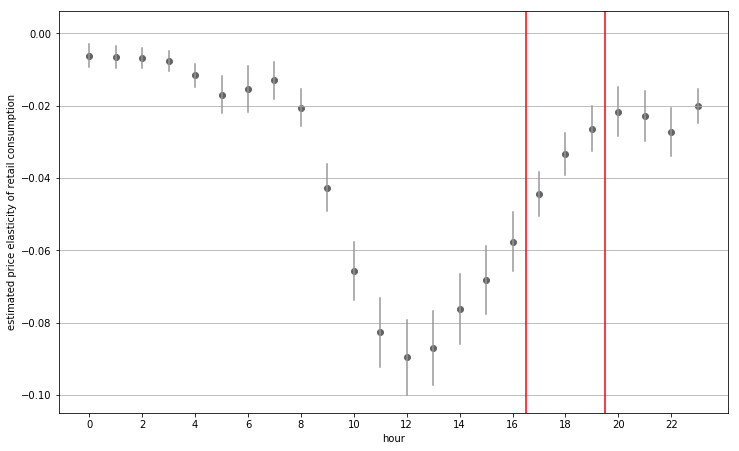
\includegraphics[width=1 \textwidth]{03_figures/r_elasticity_hour}
\end{figure}
Pooling across all 1,096 days we find that a 100 percent increase in the spot price causes a decrease in consumption of about 2.8 percent - which appears to be driven by reductions on business days. This is despite that for two of the three years none of the consumers pay the spot market price and the last year it is only offered as an option for a minority. Thus, it is a relatively surprising how responsive the consumption of households and small firms are compared to that of wholesale consumers.
\par
Reversely, one possible explanation for why we do not capture a much higher elasticity for wholesale consumption, could be that the estimations are blurred by wholesale consumers dragging the result in different direction as they are much less homogeneous than retail consumers. This would be in line with the smaller magnitude of the standard errors of the estimated elasticity for retail consumers.
\bigskip\par
There is a relatively large consumption decrease associated with $daytime$ where being before sunset implies a decrease in consumption of about 4 percent. This can be due to many non-electricity consuming leisure activities are weather and light dependent. On that note, a possible downward bias of $\widehat{\varepsilon}$ that could help explain the significant price elasticity of retail consumption would be if an unobserved variable such as sunshine correlates positively with wind power while leading to lower electricity consumption.
\begin{table}[H]
\begin{threeparttable}
  \centering
  \caption{log retail electricity consumption by region, hours 17-19 (REIV)}
  \label{tab:r_region}
  \footnotesize
    \begin{tabular}{lccccc}\toprule
                    &     (1) All   &(2) Business day   &(3) Non-business day   &     (4) DK1   &     (5) DK2   \\
                    &        b/se   &        b/se   &        b/se   &        b/se   &        b/se   \\
\midrule
log spot price      &     -0.0275***&     -0.0354***&     -0.0354***&     -0.0292***&     -0.0305***\\
                    &    (0.0056)   &    (0.0059)   &    (0.0059)   &    (0.0061)   &    (0.0092)   \\
Share time-of-use tariff&     -0.0406***&     -0.0350***&     -0.0350***&               &     -0.0069   \\
                    &    (0.0101)   &    (0.0110)   &    (0.0110)   &               &    (0.0148)   \\
Oct-Mar (Radius only)&      0.0517***&      0.0531***&      0.0531***&               &      0.0204   \\
                    &    (0.0119)   &    (0.0117)   &    (0.0117)   &               &    (0.0190)   \\
log retail meters   &      0.9077***&      0.9253***&      0.9253***&      0.8960***&      1.0056***\\
                    &    (0.0376)   &    (0.0351)   &    (0.0351)   &    (0.0369)   &    (0.0340)   \\
Temperature         &     -0.0035***&     -0.0046***&     -0.0046***&     -0.0039***&     -0.0037***\\
                    &    (0.0004)   &    (0.0005)   &    (0.0005)   &    (0.0005)   &    (0.0007)   \\
Temperature squared &      0.0001***&      0.0001***&      0.0001***&      0.0001***&      0.0001** \\
                    &    (0.0000)   &    (0.0000)   &    (0.0000)   &    (0.0000)   &    (0.0000)   \\
Daytime             &     -0.0409***&     -0.0449***&     -0.0449***&     -0.0338***&     -0.0582***\\
                    &    (0.0030)   &    (0.0030)   &    (0.0030)   &    (0.0018)   &    (0.0040)   \\
Time variables      &         Yes   &         Yes   &         Yes   &         Yes   &         Yes   \\
\midrule
\(R^2\) within      &      0.8086   &      0.8152   &      0.8152   &      0.7923   &      0.8866   \\
\(R^2\) between     &      0.9930   &      0.9933   &      0.9933   &      0.9927   &      0.9963   \\
Number of groups    &          48   &          48   &          48   &          39   &           9   \\
Obs. per group      &       3,288   &       2,205   &       2,205   &       3,288   &       3,288   \\
\bottomrule\end{tabular}

    \begin{tablenotes}
    \item Robust Robust standard errors are clustered at grid level and reported in parentheses. * p<0.10, ** p<0.05, *** p<0.01.
    \item Log spot price is instrumented for by wind power prognosis for the same region.
  \end{tablenotes}
\end{threeparttable}
\end{table}
%More homogenous consumers => mainly residential.
%Kommenter - clustering på 9 grids er måske lidt lidt... -> Driver at vi opnår så lavt et resultat
\subsubsection{Results for Radius}
We examine the grid company Radius separately. Radius operates in the Copenhagen metropolitan area and since December 2017 its flex-settled customers (households and small companies) are charged a Time-of-Use (TOU) tariff of 0.835 DKK (0.112 EUR) for the hours 17-19 from October until March and 0.3236 DKK (0.043 EUR) otherwise. Table \ref{tab:r_radius} shows pooled 2SLS estimates of electricity consumption for households and small companies in Radius for the hours 17, 18, and 19.
\par
The estimated effect of this tariff is found to be a decrease in electricity demand of 2.2 percent for the hours when it is relevant. However, on business days the smaller effect of 1.4 percent is only statistically significant at the 10\% level while the decrease is no less than 4.1 percent on non-business days where it can be easier to alter consumption patterns simply because there are more non-work hours free to shift consumption to.
\begin{table}[H]
\centering
\begin{threeparttable}
  \vspace{-0.0cm}
  \caption{log retail electricity consumption in Radius, hours 17-19 (P2SLS)}
  \label{tab:r_radius}
      \footnotesize
  \begin{tabular}{lccc}
        \begin{tabular}{lccc}\toprule
                    &(1) All days   &(2) Business days   &(3) Non-business days   \\
                    &        b/se   &        b/se   &        b/se   \\
\midrule
log spot price      &     -0.0184** &     -0.0251***&      0.0061   \\
                    &    (0.0076)   &    (0.0081)   &    (0.0179)   \\
Share time-of-use tariff&     -0.0219***&     -0.0137*  &     -0.0408** \\
                    &    (0.0081)   &    (0.0080)   &    (0.0174)   \\
log retail meters   &     -1.6012*  &     -1.2890   &      0.3618   \\
                    &    (0.8606)   &    (0.9208)   &    (1.6832)   \\
Temperature         &     -0.0029***&     -0.0040***&     -0.0026** \\
                    &    (0.0006)   &    (0.0007)   &    (0.0013)   \\
Temperature squared &      0.0000   &      0.0000   &     -0.0000   \\
                    &    (0.0000)   &    (0.0000)   &    (0.0000)   \\
Daytime             &     -0.0450***&     -0.0450***&     -0.0250   \\
                    &    (0.0104)   &    (0.0108)   &    (0.0198)   \\
Time variables      &         Yes   &         Yes   &         Yes   \\
\midrule
Adj. \(R^2\)        &      0.9462   &      0.9587   &      0.9297   \\
Observations        &       3,288   &       2,205   &       1,083   \\
\bottomrule\end{tabular}

  \end{tabular}
    \begin{tablenotes}
        \item  Robust Robust Robust standard errors are clustered at grid level and reported in parentheses. * p<0.10, ** p<0.05, *** p<0.01.
         \item Log spot price is instrumented using the wind power prognosis.
    \end{tablenotes}
  \vspace{-0.0cm}
  \end{threeparttable}
\end{table}


\subsection{The validity of instrumenting}
\label{subsec:r_validity}
All our statistical test results are reported in appendix \ref{app:statistical_tests}. As they are first and foremost regarding the validity of instrumenting for the log spot price by wind power prognosis we choose to do the tests based on POLS and P2SLS procedures separately for the biggest grid company in each price region as more elaborate test methods are developed and implemented into the core of Stata for these techniques compared to RE and REIV procedures \citep{statacorp2017stata}.
\bigskip\par
For single-grid estimations we use robust standard errors as well, as the simultaneous Breusch-Pagan / Cook-Weisberg test for heteroskedasticity clearly rejects the $H_0$ of homoscedasticity $(p=0.000)$. However, specifically for Radius in DK2 the Bonferroni-adjusted p-values for price, number of wholesale meters, and temperature are $\sim1$, shows that they are quite homoscedastic while heteroscedasticity is caused by seasonality and daily patterns.
 (appendix \ref{app:homoscedasticity}).
\bigskip\par
Different specifications for the reduced form estimation of log spot price can be seen in table \ref{tab:reduced_form_price_dk1} for DK1 and equivalently in table \ref{tab:reduced_form_price_dk2} in appendix \ref{app:relevance} for DK2. The clear relevance of wind power prognosis in the same region as an instruments for the spot price stands out. Not only due to the high significance of the estimate in column for (3) but even more so from the great reduction in the adjusted $R^2$ value by .09 for DK1 and .07 for DK2 when having omitted wind power prognosis in column (4) relative to column (3).
%\par % Er næste par nødvendig? 
%Though the effect of a given absolute change in the wind power prognosis is almost 3 times as high for DK2, this is more than offset by both the mean and standard deviation of wind power prognosis 3$\frac{1}{2}$ times higher for DK1 (table \ref{tab:descriptive}).

\begin{table}[H]
\begin{threeparttable}
  \centering
  \caption{Reduced form of log spot price for DK1, business days, hours 11-15 (POLS)}
  \label{tab:reduced_form_price_dk1}
  \footnotesize
  \begin{tabular}{lcccc}
         \begin{tabular}{lcccc}\toprule
                    &(1) 3 instruments   &(2) DK1 and DK2   &     (3) DK1   &    (4) None   \\
                    &        b/se   &        b/se   &        b/se   &        b/se   \\
\midrule
Wind power prognosis same region&     -0.0920***&     -0.0951***&     -0.1617***&               \\
                    &    (0.0137)   &    (0.0130)   &    (0.0079)   &               \\
Wind power prognosis other region&     -0.2727***&     -0.2724***&               &               \\
                    &    (0.0478)   &    (0.0479)   &               &               \\
Wind power prognosis for Sweden&     -0.0048   &               &               &               \\
                    &    (0.0057)   &               &               &               \\
log wholesale meters&     -0.6420   &     -0.6021   &     -1.0020   &               \\
                    &    (0.9546)   &    (0.9505)   &    (0.9144)   &               \\
Temperature         &     -0.0236***&     -0.0238***&     -0.0235***&      0.0001   \\
                    &    (0.0033)   &    (0.0033)   &    (0.0034)   &    (0.0001)   \\
Temperature squared &      0.0008***&      0.0008***&      0.0008***&     -0.0000***\\
                    &    (0.0001)   &    (0.0001)   &    (0.0001)   &    (0.0000)   \\
Time variables      &         Yes   &         Yes   &         Yes   &         Yes   \\
\midrule
Adj. \(R^2\)        &      0.4604   &      0.4605   &      0.4550   &      0.9480   \\
Observations        &       3,675   &       3,675   &       3,675   &       3,675   \\
\bottomrule\end{tabular}

  \end{tabular}
    \begin{tablenotes}
        \item Robust standard errors are in parentheses. * p<0.10, ** p<0.05, *** p<0.01.
    \end{tablenotes}
\end{threeparttable}
\end{table}
The t- and F-tests deem the wind power prognosis for DK2 to be a relevant instrument for the log spot price in DK1. Reversely, wind power in DK1 is not relevant for the price in DK2, instead the wind power prognosis for Sweden has a significant effect. The robust test of the first stage in Stata likewise clearly rejects that either of the instruments are weak \citep{statacorp2017stata}. However, the adjusted $R^2$ value barely decreases when omitting the second instrument in going from column (2) to (3); they do not carry any relevant explanatory power. This observation lead us to the conclusion that our model would be overspecified if more instruments than the wind power prognosis for the same region were included. \footnote{Wooldridge's robust score test and the robust regression-based test show that log spot price is endogenous when instrumenting by wind power prognosis in the other region (for DK1) or wind power prognosis for Sweden (for DK2). However, Wooldridge's heteroscedasticity-robust score test of overidentifying restrictions is only barely rejected for DK1 and clearly rejected for DK2 (appendix \ref{app:endog_overid}), \citep{statacorp2017stata}.}

\subsection{Heterogeneity and robustness}
\label{subsec:r_robustness}
We conduct a number of additional estimations to evaluate the robustness of the results above. Checks for wholesale consumption are included in appendix \ref{app:robustness_wholesale}, while those for retail are reported in appendix \ref{app:robustness_retail}. We estimate sample split results of our specification \eqref{eq:baseline} by the two price regions and for each year.
\bigskip\par
For wholesale consumption estimates are reported in table \ref{tab:ws_region_year}. It appears that the overall response is likely to be driven by DK1 (Western Denmark) whereas estimates for DK2 are small and insignificant. It should, however, be noted that there are only 9 grid companies in DK2 which may boost the grid-clustered standard errors upwards. Also the 9 companies enter with equal weight even though the price region is clearly dominated by Radius and Cerius as is evident from appendix \ref{app:grids}.
\par
Though the estimated elasticity varies a lot between the months as seen in figure \ref{fig:ws_elasticity_month}, results are, however, quite robust across years. Here we cannot reject that estimates differ.
\par
We consider the five largest grid-areas (in terms of the number of meters) separately in table \ref{tab:ws_grids_large}. Here estimates differ quite significantly which suggests there are some unobservable heterogenous characteristics that can explain the different responses to price changes. For example the estimated elasticity for Cerius, albeit small in magnitude, is significantly positive for which we can think of no other reason than omitted variable bias.
\bigskip\par
For retail consumption there is no significant difference in the price elasticity between the price regions (table \ref{tab:r_region}). Though we would expect the elasticity to be higher in 2018 compared to 2016, there is no significant difference here either (table \ref{tab:r_year}).
\par
To further examine the robustness of the estimated effects from the time-of-use tariff and to control for this effect we have included the variable in the REIV estimations shown in table \ref{tab:r_region}, controlling for the grid-specific consumption pattern of Radius by a control indicating months October-March and grid company Radius. Here the estimated effect of the TOUT use is significant and of slightly greater magnitude compared to our estimates for Radius alone.
\bigskip\par
Our overall estimates of the price elasticity for wholesale and retail consumption remain largely robust, but also motivates a closer look at more disaggregated data to examine the drivers of the observed heterogeneities.
\par

\subsection{Discussion}
\label{subsec:r_discussion}
Our estimates are bigger than those obtained by \citet{lijesen2007real} but around the same size as \citet{wolak2001impact} finds for 5 of the 6 most elastic industries. Part of this difference has to do with limited access to disaggregated high frequency data. Although estimates are statistically significant their economic significance is more limited. They all point to a quite inelastic electricity demand even for the most elastic part of the market. This suggests that the prospects of using decentralized interventions such as demand response programs are limited. From the small estimated effect on the time-of-use tariff in Radius similar conclusions can be conjectured. Prices does, however, rise quite dramatically during hours of peak demand. Thus, rather small decreases in consumption can still matter. %Vores resultater er yderligere begrænset af at der i vores specifikation antages konstant elasticitet.
\bigskip

Oddly enough, the time-of-use tariff did seem to have an effect outside of the area that was actually affected by the tariff. This could be a response from an increasing awareness that electricity demand and thus emissions from production are high in the peak period. Likewise, awareness about the fact that electricity supply largely relies on coal power when the wind is calm could be the driver of the general elasticity as few retail consumers actually pay an hourly price.
\par
Even though people do not appear to respond much to electricity prices nor the TOUT this could simply be due to little available information. The tariff is applied grid wide, but its actual implementation (into billing contracts etc.) is left for the individual electricity providers to decide on. Thus, both information granted and actual exposure to the tariffs may vary significantly across providers. It could also simply be the case that people have not had enough time to adjust their behavior, which can be costly in terms of utility. Adjustment time may similarly also depend on the implementation of the program, this is the extent to which consumers were actually aware of the tariff introduction.
\bigskip

Even in the absence of large consumption changes there are still other advantages associated with demand responses such as real time pricing. Without load shedding the current system of limited exposure to price fluctuations is implicitly build to over-cater to peak demand which is harmful through greenhouse gas emissions and promotion of high-cost, non-competitive supply. Non-distorted prices makes up for this by better reflecting the current state of the market - at least in the absence of externalities.\footnote{In the presence of uninternalized, negative production externalities the problem of over-catering is exacerbated even more} When prices are high this encourages investments in energy efficient devices but it also makes electricity storage more profitable. Research and development of storage may, in the long run, make it feasible to rely purely on intermittent, renewable energy.
\bigskip

There could still be decentralized solutions to the issue of smoothing electricity consumption. One obvious solution would be to limit the number of contracts where consumers pay a fixed price and increase contracts with more flexible settlement. The EU are in the process of implementing a great deal of policies moving in this direction. There is, however, little empirical support of what difference implementation could make without the provision of additional information. Given that people have limited cognitive capacity it could be useful to provide cost examples of using a specific electrical device during peak compared to off-peak or shoulder periods.
Another concern here is that this could also have the opposite effect if the price provided then is perceived as too small to matter rather than exacerbate prices. If people rely on heuristics this could likely be a "harmful" rule of thumb.
\bigskip

%Section on some of the experimental evidence out there.
There is much experimental research devoted to looking into ways of getting people to conserve energy using non-standard economic tools because the standard tools does not appear to alter behavior. This paper highlights the importance of these results. Examples include \citet{allcott2011social} where US consumers are informed about how their own consumption of energy compares to that of their neighbours which especially causes those with a relatively high consumption to adjust it to a level closer to that of their neighbours thereby conforming to social norms. This is also an argument in favour of decentralized solutions that focus on moving the demand curve itself rather than moving customers along it. \citet{kirschen2003demand} argues that electricity is perceived as necessary, but it may be needed to change the perception of what constitutes "normal consumption". From figure \ref{fig:cons_time_series} we note that consumption is much lower in summer which reveals potential to reduce in wintertime as well despite higher requirements for electrical heating and lighting.
\par Another example is \citet{saele2011demand} where they use information in combination with a demand response mechanism. Authors find that costumers respond more than in other studies and conclude that it especially has potential for consumers with electrical heating which is not of much relevance to Denmark.\bigskip

All in all, demand responses may not be the most easily implemented and effects may not be big enough for them to stand alone. While these initiatives may be cost-effective there is limited evidence of persistent effects over time as \citet{allcott2014short} among others find that effects are decaying after treatment has ended.

\subsubsection{Centralized solutions}
Given how costly it can be for consumers to alter consumption behavior there may be a bigger need for more centralized solutions to the issue. One option could be to directly affect and alter the supplying capacities.
Increased market integration may satisfy many of these requirements. In section \ref{subsec:t_EU} it is described how better integration in terms of greater connecting capacities across the current price regions could lead to less price volatility in spite of more reliance on intermittent renewables because of a more optimal energy mix. This corresponds to diversification of the generation portfolio. Expanding grid boundaries can make an electricity production that relies on intermittent renewable sources more stable. This almost corresponds to invest across a market index which diminishes individual risk from each producer. It would allow for complementary production capacities among the energy producers. Hydro and wind energy for example complement each other well;  hydro can be deployed when the wind does not blow and then cheap wind power can be used to pump water reservoirs full again. Initiatives in this direction are already being taken at the European level with the 'Clean Energy for all Europeans' package consisting of 8 legislative acts and the renewable energy directive.
\bigskip

%Lav en overgang
Technology has thus far prevented "smart" solutions but an increasing number of countries are rolling out smart meters that allow for integration into a smart grid. A smart meter can allow for remote metering, show current consumption and current prices. In similar fashion a smart device is one where its electricity consumption can be changed automatically in response to the electricity price.
\citet{biggar2014economics} reports how end-of-use consumers are committing to make their devices capable of being responsive to the real time prices. This implies more integration of retail consumers into the wholesale market which according to our results could be a way to induce a higher price elasticity. Smart grids can be advantageous by providing a feasible way to expand electricity storage. End-of-use owned storage units (such as electrical cars) that are already readily available could be integrated onto the grid and programmed to charge whenever renewable production prices exceeds demand. Owners could then opt to sell stored electricity when demand exceeds such production.


\subsection{Possible extensions}
\label{subsec:r_extensions}
A straightforward extension would be to look at the elasticity of aggregate consumption in each price region and not only on an unweighted average of the effects in grid companies of very different size. However, this would provide less efficient estimates due to the loss of nuances between grids. As the FE estimates are identical to the RE estimates, however less efficient, we could instead try to weight the FE estimates by the average number of wholesale meters in each grid.
\bigskip\par
A more cumbersome extension could be to include various observed grid-specific effects. However, precise identification might be less feasible as the boundaries of the grids often are not in line with municipality borders or other common statistical entities. The motivation being that one can expect a exists great variation in terms of size, distribution of retail customers (residential and commercial), and industry-commercial ratio of wholesale customer. Both between grid companies and over time within a grid.
\bigskip\par
A very tractable but hard-to-come-by extension would be to use micro data which would remove the bias from compositional changes in the presence of heterogeneous consumers. Similarly more detailed data would allow for an exploration of further heterogeneities in terms of who is more or less responsive to electricity prices. This would be useful for both the wholesale market where it could be interesting to look at heterogeneity across different industries while for the retail consumers it would be interesting to explore how age, gender, or educational level affects price responsiveness.
